\chapter{Metodología}\label{cap:metodologia}

\section{Formalización de ZSD} \label{ssec:formalizaciondezsd}
Para formalizar ZSD denotamos el conjunto de las clases como $\mathcal{C} = \mathcal{S} \cup \mathcal{U}$, donde $\mathcal{S}$ son las clases vistas para entrenamiento y $\mathcal{U}$ las clases no vistas, utilizadas en la etapa de pruebas. Además se tiene que $\mathcal{S} \cap \mathcal{U} = \emptyset$. Aunque no es necesario definir el conjunto de clases de pruebas, ya que el modelo tiene que ser capás de detectar tanto clases vista como las no vista, esto se hace para poder tener una evaluación cuantitativa.

Denotamos a una imagen como $\mathcal{I} \in \mathbb{D}^{\mathcal{M} \times \mathcal{N} \times 3}$. Donde $\mathbb{D} = \{0,...,255\}$, $\mathcal{M}$  es el largo de la imagen, $\mathcal{N}$ el ancho. Esta es la forma en la que se representa cada pixel de la imagen en el formato \textbf{RGB}, donde se tiene 3 canales que caracterizan la intensidad de los colores rojo, verde y azul. 

Por cada imagen se provee un conjunto de cuadros delimitadores  $\mathbb{B} = \{b_0,...,b_k\mid b_i \in N^4\}$ y sus etiquetas asociadas como $\mathbb{Y} = \{y_0,...,y_k\mid y_i \in \mathcal{C}\}$. Para cada cuadro delimitador $b_i$ extraemos una característica profunda utilizando una red neuronal convolucional denotada como $\phi(b_i) \in \mathbb{R}^{D_1}$. 

Denotamos las incrustaciones semánticas $w_j \in  \mathbb{R}^{D_2}$ obtenido por algún modelo como Wor2Vec. El conjunto de todas las imágenes de entrenamiento se indica con $\mathcal{X}^s$, que contiene ejemplos de todas las clases de objetos visibles.  El conjunto de todas las imágenes de prueba que contienen muestras de clases de objetos invisibles se indica con  $\mathcal{X}^u$. En particular, no hay ningún objeto de clase invisible en $\mathcal{X}^s$, pero $\mathcal{X}^u$ puede contener objetos vistos.\\

El objetivo es encontrar una matriz de proyección $W_p$, tal que \[ \psi_i = W_p\phi(b_i) \:\:\:\mid\:\:\: W_P \in \mathbb{R}^{D_2 \times D_1},\:\:\: \psi_i \in \mathbb{R}^{D_2} \] Note que $\psi_i$ y las incrustaciones semánticas se encuentran en el mismo dominio. Como mencionamos en secciones anteriores, el espacio vectorial semántico, tiene una gran capacidad de capturar similitudes semánticas. Por lo cual, resulta clave encontrar una matriz que para cada cuadro delimitador se proyecte lo más cerca posible a la incrustación semántica de su clase. 

El resultado es una función 
\[f : \mathcal{X}, W_p  \to \{y_0,...,y_k\mid y_i \in \mathcal{C}\} \quad \operatorname{con}\quad \mathcal{X} =  \mathcal{X}^s \cup \mathcal{X}^u\] 
con un riesgo empírico regularizado mínimo $\mathcal{R}$ definido de la siguiente manera: 
\[ \arg_{}\min_{f \in F} \mathcal{R}(f(x,W_p))\quad, \] 
donde $x \in \mathcal{X}^s$ durante el entrenamiento. La función de mapeo utilizada en la etapa de inferencia, tiene la siguiente forma \[ f(x,W_p) = \arg_{}\max_{y \in \mathcal{C}}\max_{b \in \mathbb{B}(x)} (F(x,y,b,W_p)) \quad,\] donde los $\mathbb{B}(x)$ es el conjunto de propuestas de la imagen $x$. Intuitivamente se buscan los cuadros delimitadores de mejor puntuación y se les asigna la categoría de objeto de puntuación máxima.

\section{Arquitectura y Diseño} \label{sec:arquitecturaydiseno}

\subsection{Arquitectura} \label{ssec:arquitectura}
\begin{figure}
	\centering
	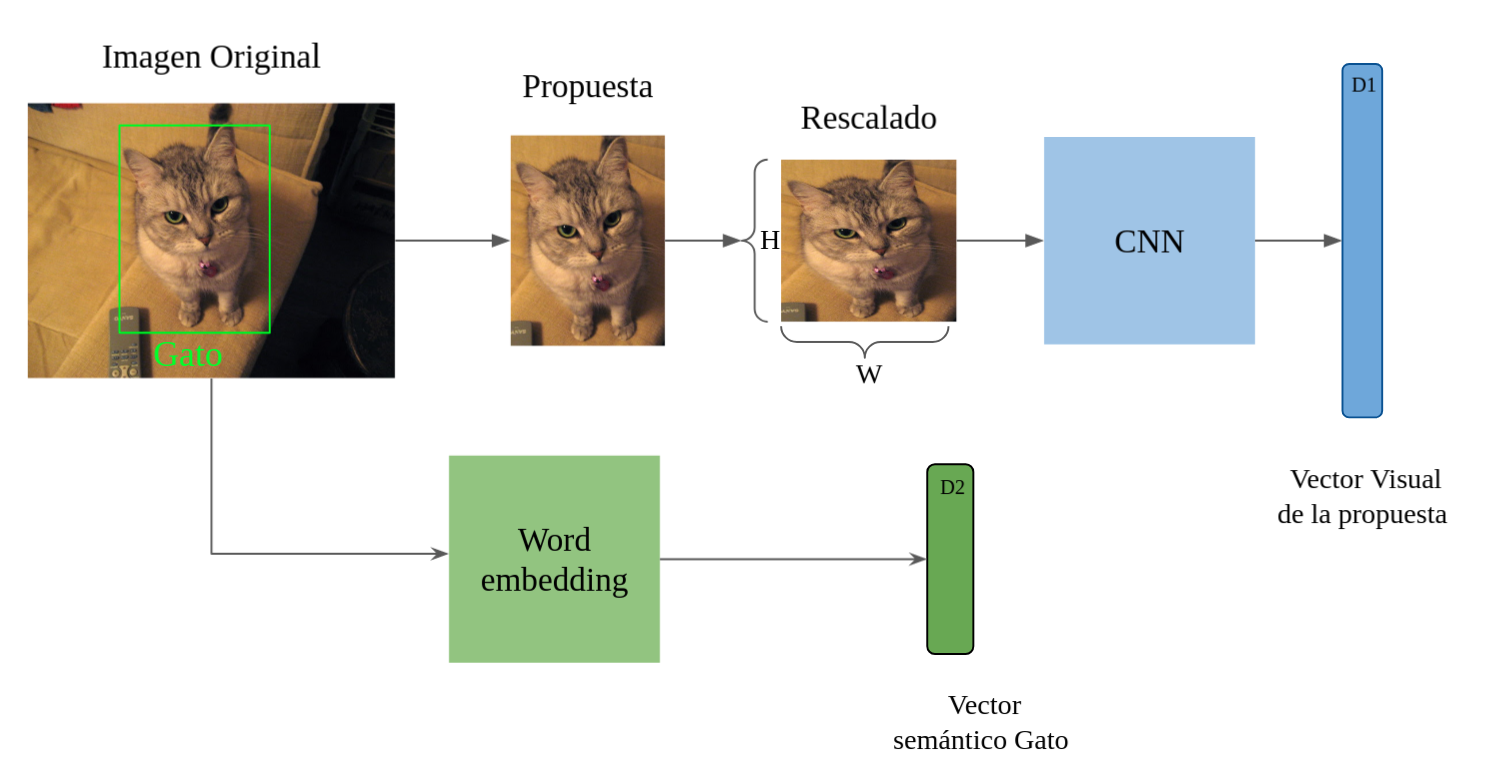
\includegraphics[width=0.9\textwidth]{img/arquitectura.png}
	\caption{Arquitectura propuesta para ZSD, utilizando incrustaciones semánticas y visuales, ademas se muestra la dimensión en cada paso.}
	\label{fig:arqutectura}
\end{figure}
Como se menciono anteriormente, hemos decido basarnos en el modelo propuesto por Bansal \etal~\cite{bansal2018zero} para abordar el problema de ZSD. La arquitectura propuesta en este  trabajo se puede dividir en las siguientes etapas:
\begin{itemize}
	\item \textbf{Pre-procesamiento:} Se recorren todas las imagen de entrenamiento y se extrae una característica profunda por cada cuadro delimitador, utilizando una red neuronal convolucional. Éste se asocia con el vector semántico de la clase que tiene asignada el cuadro, que se puede obtener con modelos de incrustación de palabras previamente entrenados, como Glove o Word2vec. Esta etapa nos genera como salida dos listas 
	\[X = [\phi(b_0),...,\phi(b_k) \mid \phi(b_i) \in \mathbb{R}^{D_1}]\] 
	\[W = [w_0,...,w_k \mid w_i \in \mathbb{R}^{D_2}]\]
	
	\item \textbf{Entrenamiento:} Utilizamos el espacio de incrustación común (${R}^{D_2}$) para calcular una medida de similitud entre las proyecciones  $\phi(b_i)$ y los vectores densos de palabras $w_i$. Luego, se entrena la proyección usando una función de pérdida, que impone la restricción que el puntaje de la similitud de un cuadro delimitador, con su clase verdadera, debe ser más alto que el de otras clases. 

	La función de pérdida definida como: 
	
	\[\mathcal{L}(\psi_i, w_i) = \sum_{j \in \mathcal{S}, j\neq i} max(0, m - S_{ii} + S_{ij})\] 
	donde $m$ es el margen máximo, y $S_{ij}$ es la similitud entre la proyección $i$-$esima$ y la incrustación $j$-$esima$.
 
	También se agrega una función de pérdida de reconstrucción como sugieren Kodirov \etal~\cite{kodirov2017semantic}. Se utilizan las características del cuadro delimitador proyectadas para reconstruir las características profundas originales, y calcular la pérdida de reconstrucción como la distancia $L2$  entre la característica reconstruida y la característica profunda original.
	\[\mathcal{L}_r = \Vert{\phi(b_i) - \psi_iW_p^T}\Vert^2 \] 
	Luego, definimos $\lambda$ como un coeficiente de ponderación que controla la importancia del primer y segundo término, que corresponden a las pérdidas de proyección y reconstrucción respectivamente. Por lo cual la función de perdida total es: 
	\[\mathcal{L}_t = \lambda \mathcal{L} + (1-\lambda) \mathcal{L}_r \]
 	 
 	En la \autoref{fig:arqutectura} se puede apreciar la arquitectura completa propuesta en este trabajo.
 	 
 	\item \textbf{Evaluación:} Por cada imagen de entrenamiento se genera un conjunto de propuestas de cuadros delimitadores. Luego, se eliminan todos los que no tienen un puntaje de confianza mayor a un umbral $t$. Para cada cuadro obtenido se computa la característica profunda $\phi(b_i)$ y utilizando la matriz de proyección $W_p$, se predicen las característica semánticas. Por último, se calcula la similitud con las características semántica de todas clases invisibles, asignando al cuadro delimitador la que tenga mayor puntaje.
\end{itemize}

Es común que en la detección de objetos se incluya una clase de fondo, para obtener un detector robusto que pueda discriminar eficazmente entre objetos de primer plano y objetos de fondo. En ZSD, esto no es un problema trivial, ya que no se sabe si un cuadro de fondo incluye elementos como cielo, tierra, bosque, etc. o una instancia de una clase de objeto invisible. En muchos trabajos se proponen distintas técnicas para abordar este problema, pero no presentan mejoras en evaluaciones cuantitativas. Es por esto que no se incluye una arquitectura que discrimine cuadros de fondos.

\subsection{Conjuntos de datos} \label{ssec:conjuntosdedatos}
\textit{Common Objects in Context} (COCO) es una base de datos que tiene como objetivo ayudar en la investigación de detección de objetos, posee varias caracteristicas como segmentación de instancias, subtítulos de imágenes y localización de puntos clave de personas. Este conjunto de datos contiene 91 tipos de objetos o  clases, con un total de 2.5 millones de instancias etiquetadas en 328.000 imágenes.

La gran cantidad de instancias de objetos y de categorías, resulta en un conjunto ideal para entrenar y evaluar modelos de ZSD. Además, la mayoría de la imágenes consta de una gran cantidad de objetos, a diferencia de conjuntos como Visual Genome. Esto generan un contexto en el que varios objetos se relacionan y se superponen, emulando de una mejor manera situaciones de la vida real. 

En este trabajo se utilizan las imágenes de entrenamiento del conjunto COCO 2014 e imágenes del conjunto de validación para realizar las pruebas de ZSD.
\begin{figure}
	\begin{center}
		\centering
		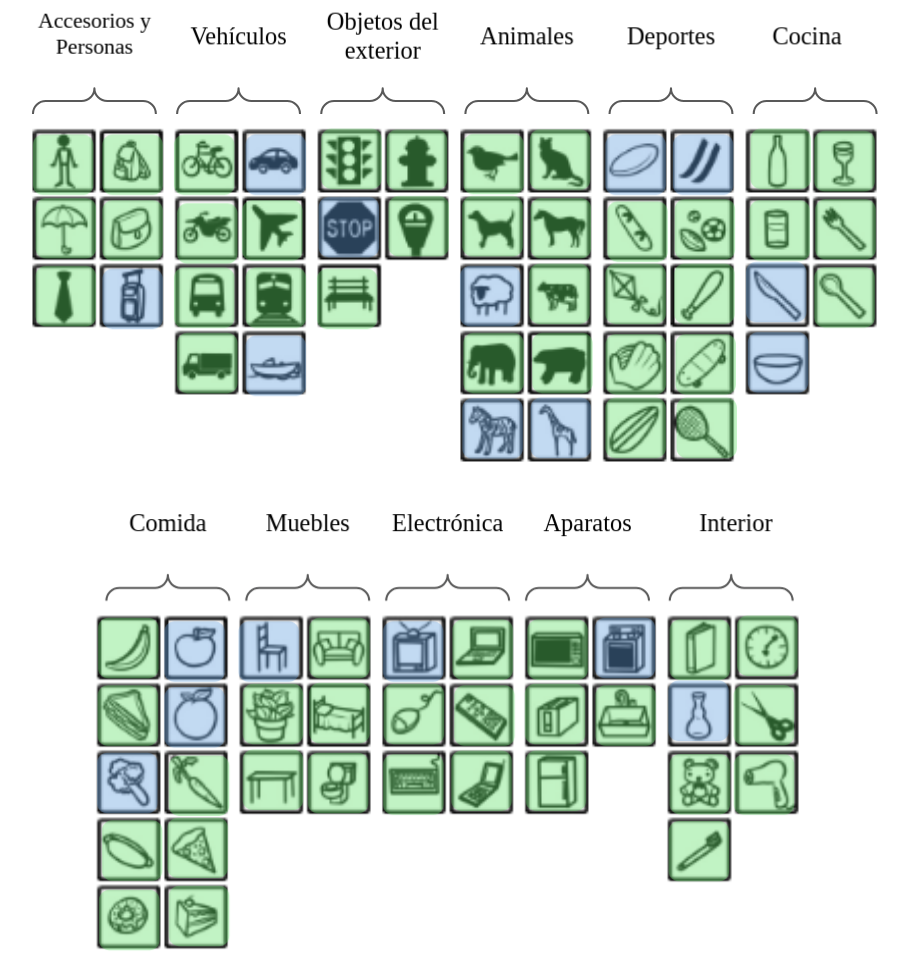
\includegraphics[width=1\textwidth]{img/data_set.png}
		\caption{División de las clases para entrenamiento (verde) y pruebas (azul).}
		\label{fig:data_set}
	\end{center}	
\end{figure}

Como COCO no provee una separación de los datos para evaluar modelos de ZSD, es necesario crear una forma de dividir las clases en vistas e invisibles. Esta separación resulta de suma importancia, ya que se debe cumplir que para todo objeto del conjunto prueba, exista otro de aspecto similar que este presente durante el entrenamiento. Además, no se puede encontrar ningún objeto de prueba en los datos de entrenamiento. Para esto, se aprovecha de que COCO tiene agrupadas las clases por ``Clases superiores'', y de cada uno de estos grupos se elige de forma aleatoria un 70\% de clases para entrenamiento y un 30\% para pruebas. Es decir, 47 y 18 clases respectivamente, de un total de 65 clases de COCO 2014. En la \autoref{fig:data_set} se puede observar el resultado de esta división. Por último se eliminaron todas las imágenes de entrenamiento que contengan al menos una instancia de las clases de prueba. Esto resulta en 42564 imágenes con 261258 instancias de entrenamiento, y 3008 imágenes con 10878 instancias de prueba. 

Bansal \etal~\cite{bansal2018zero}, divide el conjunto de datos de manera similar, utilizando la misma cantidad de clases para las etapas de prueba y entrenamiento. Pero la diferencia radica en que utiliza los vectores densos de palabras para agrupar las clases, utilizando la  similitud coseno entre los vectores como métrica. Por último, elige de forma aleatoria las clases visibles e invisibles de cada grupo. En este trabajo también se utiliza esta separación, para logra una comparación de modelos más justa.

\begin{figure}[H]
	\begin{center}
	\begin{subfigure}{.3\textwidth}
		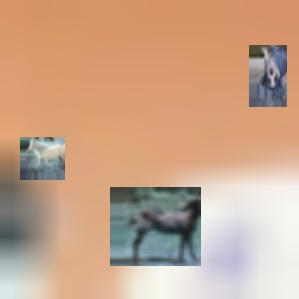
\includegraphics[width=1\textwidth]{img/cifar-zsd-test400.jpg}
		\label{fig:ex1}
	\end{subfigure}
	\begin{subfigure}{.3\textwidth}
		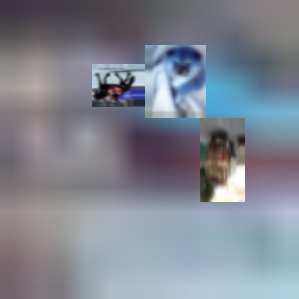
\includegraphics[width=1\textwidth]{img/cifar-zsd-test379.jpg}
		\label{fig:ex2}
	\end{subfigure}
	\begin{subfigure}{.3\textwidth}
		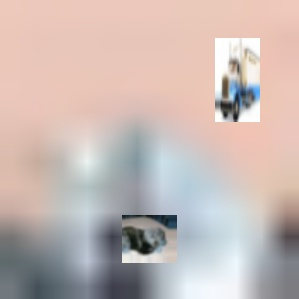
\includegraphics[width=1\textwidth]{img/cifar-zsd-test283.jpg}
		\label{fig:ex3}
	\end{subfigure}
	\caption{Ejemplos de imágenes del conjunto de datos CIFAR-ZSD.}
	\label{fig:CIFAR-ZSD}
	\end{center}
\end{figure}

COCO puede resultar pesado en término computacional. Para soluciona esto se creó un conjunto de datos sintético basado en CIFAR-100 datasets, el cual denominamos CIFAR-ZSD. Éste consta de imágenes localizadas, rotadas y re-escalada aleatoriamente con un fondo de otra imagen (algunos ejemplos se pueden ver en la \autoref{fig:CIFAR-ZSD}). Con esto se intenta simular imágenes reales en la cual un objeto puede aparecer con distintos aspectos y escalas. Este conjunto esta dividido para que ninguna instancia de prueba  aparezca en el conjunto de entrenamiento.

Aunque este conjunto resulta muy útil para hacer pruebas de modelos, no es bueno para reportar métricas reales, pero en combinación con COCO, que si lo es, ayudan a enfrentar el problema de ZSD de una forma más práctica.

\subsection{Detalles de la implementación} \label{ssec:detallesdelaimplementacion}

El paper de Bansal \etal~\cite{bansal2018zero}, carece de una implementación de acceso público, por lo cual, se realizó una implementación propria, basándose en los detalles que se pueden extraer del documento publicado. Fue necesario realizar algunas suposiciones, pero también, nos otorgo flexibilidades a la hora de codificar. Se buscó obtener resultados lo más cercanos posibles a los reportados, siendo fiel a la información disponible. Para esto se decidió utilizar Python 3 con el framework Keras ejecutadose sobre TensorFlow.\\

Primero se realiza un preprocesamiento a todas las imagines del conjunto de datos de entrenamiento, que consiste en generar propuestas de objetos utilizando \textit{Edge Boxes} o \textit{Selective Search}. En la \autoref{cap:experimentos} se muestran los resultados de cada algoritmo. Luego por cada propuesta se calcula la intersección sobre unión con todos los cuadros delimitadores verdaderos. Si el IoU $> 0.5$ con algún cuadro verdadero, se guarda la propuesta y se la asocia con la clase del cuadro delimitador verdadero. Este preprocesamiento aumenta significativamente la cantidad de instancias para la etapa de entrenamiento, que resulta en un total de 1.436.835 instancias para COCO y 137.204 para CIFAR-ZSD. El siguiente paso consiste en generar el vector de características visuales y semánticas de cada cuadro delimitador. Como las CNN, utilizan un tamaño de entrada fijo, es necesario rescalar todos los cuadros.  Para \textit{VGG16} utilizamos $224 \times 224$, y en \textit{Inception ResNet V2} $299 \times 299$, que son las dimensiones por defecto. El tamaño del vector de salida de cada red es de 512 en VGG y 1536 ResNet. Para ambas usamos pesos preentrenados en Imagenet. Este paso es diferente a como se hace en el artículo de Bansal \etal~\cite{bansal2018zero}, ya que en este trabajo el modelo se entrena de extremo a extremo, es decir los pesos de la CNN se ajustan en la etapa de entrenamiento. Para obtener las características semánticas, utilizamos \textit{Word2Vec} previamente entrenado por \textit{Google News 300}. Este incluye vectores para un vocabulario de 3 millones de palabras y frases, entrenado en aproximadamente 100 mil millones de palabras de un conjunto de datos de Google News. La longitud del vector resultante es de 300. Luego se guardan dos archivos por cada imagen, en uno se encuentran los vectores visuales de cada clase y en el otro los semánticos.\\

Por último, para el entrenamiento, se creo una red con una sola capa oculta, una capa de entrada del tamaño del vector de características visuales, y una capa de salida de la dimensión de las características semánticas. Lo cual resulta en 153.900 parámetros entrenables con \textit{VGG16} y 461.100 con \textit{Inception ResNet V2}. Para esta etapa, se utilizó el optimizador Adam, un taza de aprendizaje de 10e-3, un tamaño del lote de 64 muestras y no se uso ninguna activación. Para la función de perdida se uso un lambda de 10e-3 y un margen máximo de 1.\\


\section{Experimentos}\label{cap:experimentos}

\subsection{Experimentación con propuesta de objetos} \label{ssec:experimentacionconpropuestadeobjetos}
Como se mencionó anteriormente, el número de propuestas es un parámetro clave. Algunas métricas son muy sensible a la cantidad de propuestas, afectando así los resultados finales. Esto se observó cuando se obtuvieron las primeras métricas, donde los valores estaban muy lejos de los esperados, y a medida que se aumentaba la cantidad de propuestas, los resultados empeoraban. Por este motivo, se probaron dos algoritmos (\textit{Edge Boxes} y \textit{Selective Search}), con algunas combinaciones de sus parámetros, con el objetivo de obtener una cantidad de propuestas que se superponga con el mayor número de objetos sin afectar las métricas.\\

Para no sesgar el experimento con los datos de prueba, se definió la metodología de la siguiente manera: por cada imagen de entrenamiento se corrió el generador de propuestas, y se calculó el tiempo y la cantidad de cuadros verdaderos que tenían un IoU $> 0.5$, con algún cuadro verdadero. El tiempo es un parámetro importante ya que algunos algoritmos soy muy lentos y resultan imposible de usar. 

Como se puede observar en la \autoref{tabla:edgeVSselct}, \textit{Selective Search} obtiene una mayor cantidad de superposición, pero con un número exageradamente grande de propuestas, por lo que la mejor opción es usar \textit{Edge-boxes}. En cuanto número de propuestas totales, resulta más conveniente entre 100 y 500 propuestas como máximo, ya que al aumentar este numero no se generan mejoras en superposición pero si aumenta el número de propuestas. Si tenemos en cunta el tiempo, resulta mejor \textit{Edge-boxes}, ya que demora una fracción de lo que tarda \textit{Selective Search}.\\

\begin{table}[]
	\centering
	\resizebox{12.5cm}{!} {
		\begin{tabular}{|l|c|r|r|r|c|r|}
			\hline
			\textbf{}                     & \multicolumn{4}{c|}{\textbf{Edge Boxes}}                                                                                                   & \multicolumn{2}{c|}{\textbf{Selective Search}}               \\ \hline
			\textbf{Algoritmo}            & \multicolumn{4}{c|}{\textbf{-}}                                                                                                            & \textbf{Single}         & \multicolumn{1}{c|}{\textbf{Fast}} \\ \hline
			\textbf{Numero de propuestas} & \textbf{100}                 & \multicolumn{1}{c|}{\textbf{500}} & \multicolumn{1}{c|}{\textbf{1000}} & \multicolumn{1}{c|}{\textbf{5000}} & \textbf{$\approx$ 5000} & \multicolumn{1}{c|}{\textbf{$\approx$ 1000}}  \\ \hline
			Tiempo promedio (s)           & \multicolumn{1}{r|}{0.11}    & 0,11                              & 0.12                               & 0,12                               & \multicolumn{1}{r|}{5,48}   &         1,41                           \\ \hline
			Propuetas Totales             & \multicolumn{1}{r|}{4.415.244} & 22.050.071                          & 43.802.935                           & 161.809.194                          & \multicolumn{1}{r|}{350.535.591}   &   95.643.172                                 \\ \hline
			Propuestas con IOU $> 0.5$    & \multicolumn{1}{r|}{86.233}   & 133.942                            & 155.584                             & 194.891                             & \multicolumn{1}{r|}{221.551}   & 203.563                                   \\ \hline
		\end{tabular}
	}
	\caption{Resultados de correr los distintos algoritmos de propuestas de regiones en los datos de entrenamiento. El número de propuestas verdaderas es 261.258.}
	\label{tabla:edgeVSselct}
\end{table}


\subsection{Experimentación con CNN} \label{ssec:experimentacionconcnn}
% para generar tablas de latex
\begin{figure}
	\centering
	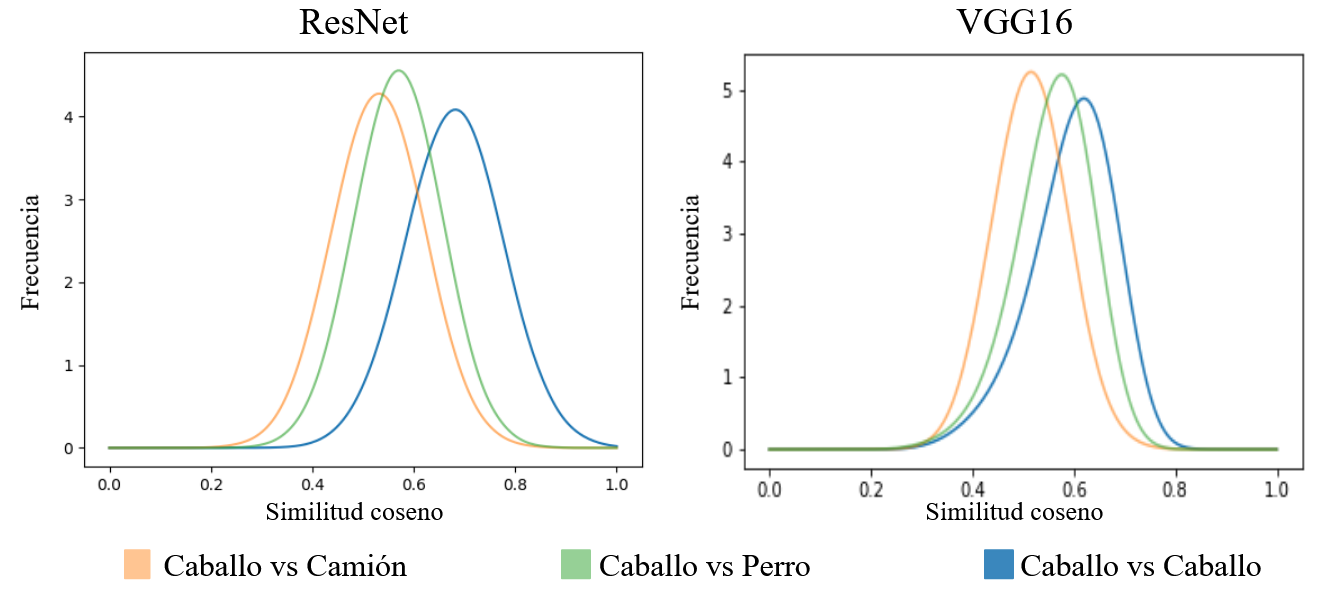
\includegraphics[width=1\linewidth]{img/vgg-vs-resnet}
	\caption{Frecuencia de la similitud coseno de los vectores de caracteristicas visuales, ente la misma y distintas clases, para las CNN  \textbf{Inception ResNet V2} y \textbf{VGG16}.}
	\label{fig:vgg-vs-resnet}
\end{figure}

Se decidió analizar la CNN ya que el modelo final es muy dependiente de esta red y de su capacidad de extraer características visuales. Lo que se quiere aquí es que la red sea capaz de asociar las caracteristicas visuales de objetos similares, y diferenciar los elementos de distinta naturaleza. En otras palabras, el espacio resultante tiene que distribuirse de tal manera que, por ejemplo, las imágenes de los animales estén muy cerca y a su ves alejadas de vehículos o electrodomésticos, pero también mantengan una separación entre los distintos animales como perro y gato. Bansal \etal~\cite{bansal2018zero} propone utilizar \textit{Inception ResNet V2}, el problema de esta red es que puede resultar pesada en cuanto a tiempo de ejecución y memoria. Por este motivo se decidió intentar con \textit{VGG16}, que reduce el número de parámetros en las capas convolucionales y mejorar el tiempo de ejecución, además es una de la más utilizada.\\

El experimento consistió en comparara miles de recuadros de 3 clases de entrenamiento, caballo, perro y camión.  Por cada cuadro se generó el vector de caracteristicas visuales. Luego se comparó utilizando la similitud coseno, entre todas las caracteristicas de caballo vs caballo, caballo vs camión y caballo vs perro. En la \autoref{fig:vgg-vs-resnet} se graficaron las frecuencias de los resultados para cada CNN. Con esto se intenta observar como se distribuyen en el espacio visual las distintas clases. Como se esperaba, la similitud entre entre animales es más grande que con un vehículo. Se observó que para \textit{Inception ResNet V2} existe una mayor separación entre clases, aunque sus similitudes están más dispersas. \textit{VGG16} parece tener una menor dispersión, pero la similitud coseno entre distintas clases tiene valores muy cercanos. Esto puede afectar de manera negativa ya que camión y caballo no poseen una gran diferencia y el modelo podría interpretarlo como clases similares.\\


\subsection{Definición de métricas} \label{ssec:definiciondemetricas}
Entre los diferentes conjuntos de datos anotados, utilizados por los desafíos de detección de objetos y la comunidad científica, la métrica más común utilizada para medir la precisión de las detecciones es el  \textit{Mean Average Precision (mAP)}, seguida por \textit{Recall}. Un problema que tienen la métricas en detección de objetos, es la fata de una implementación estándar para calcularlas. Además, aquellas implementaciones públicas están muy encapsuladas al código, y resulta muy difícil adaptarlo para medir rendimientos de modelos propios. Como ya se mencionó anteriormente, el código de Bansal \etal~\cite{bansal2018zero} no esta disponible, por este motivo fue necesario encontrar alguna implementación de estas métricas. A partir de estas búsqueda se encontraron varias opciones, sin embargo los resultados variaban mucho de un código a otro. Esto se debe a la falta de consenso en diferentes trabajos e implementaciones de AP, que es un problema al que se enfrentan las comunidades académicas y científicas, tal como se plantea en artículo de Padilla \etal~\cite{padilla2020survey}. Además, propone una definición y un código para estandarizar las métricas, de manera que se puedan comprar distintos modelos de una forma ``justa''. Por estos motivos decidimos utilizar este trabajo y su implementación para calcular nuestras métricas, aunque los resultados no den exactos a los reportados por Bansal \etal~\cite{bansal2018zero}.\\

Ahora definamos las métricas, basándonos en el trabajo \cite{padilla2020survey}. Primero es necesario estandarizar:
\begin{itemize}
	\item Falso negativo (\textbf{FN}): Para un cuadro delimitador verdadero no se obtuvo ninguna detección en absoluto, o una propuesta tiene IoU $> umbral$ con algún cuadro verdadero y no se predijo correctamente la clase.
	\item Falso positivo (\textbf{FP}): Una propuesta predijo correctamente la clase de un cuadro delimitador verdadero pero el IoU $< umbral$, o es un predicción duplicada, es decir, ya se marco otra con mayor IoU como \textbf{TP}, o se detecto un objeto inexistente con IoU $< umbral$ para todo cuadro verdadero.
	\item Verdadero positivo (\textbf{TP}): Una propuesta predijo correctamente la clase y obtuvo un IoU $> umbral$ con algún cuadro verdadero.
	\item Verdadero negativo (\textbf{TN}): Esto sólo tiene sentido si se quisiera medir propuestas que no tienen un IoU $> umbral$ con todos los cuadros verdaderos, y además se predijo como clase de fondo. Pero en este trabajo no es utilizada.
\end{itemize}
El umbral por lo general es 0.5, pero se puede cambiar para exigir que tenga una mayor superposición.\\

La \textit{Recall}, también conocida como sensibilidad, mide la probabilidad de que los objetos verdaderos (los que se encuentran en la imagen) se detecten correctamente, viene dado por: 

\begin{equation}
	\label{eqn:recall}
	Recall =\frac{TP}{FN+TP}
\end{equation}

El trabajo de Bansal \etal~\cite{bansal2018zero}, define \textit{Recall} de la siguiente manera: 
\begin{center}
	\textit{``Un cuadro delimitador predicho se marca como verdadero positivo solo si tiene una superposición de IoU mayor que un cierto umbral t con un cuadro delimitador de verdadero y no se ha asignado ningún otro cuadro delimitador de mayor confianza al mismo cuadro de verdadero. De lo contrario, se marca como falso positivo.''}\\
\end{center}

Según esta definición solo se tienen en cuenta los objetos que tuvieron al menos una propuesta con un IoU $> 0.5$, y el resto quedan fuera del cálculo de esta métrica. Esto genera una diferencia enorme entre los resultados calculados con esta definición y con los obtenidos usando la \autoref{eqn:recall}. Esto dificulta la tarea de comprar con otros modelos, con lo cual es en este trabajo reportamos ambas formas. 

Bansal \etal~\cite{bansal2018zero} además calcula una variación denominada \textit{K@Recall}, donde sólo se tienen en cuentan las \textit{K} mejores propuestas basándose en la confianza de la predicción y el resto son descartadas.\\


\textit{AP}, es una métrica popular para evaluar la precisión de los detectores de objetos mediante la estimación del área bajo la curva (AUC), que viene dada por la relación de la \textit{precisión} y la \textit{recall}. Donde la precisión consiste en medir el porcentaje de predicciones positivas correctas entre todas las predicciones realizadas y se define como:

\begin{equation} 
\label{eqn:precision}
Precision =\frac{TP}{FP+TP}
\end{equation}


Para dibujar la curva AUC necesitamos obtener múltiples pares de valores de \textit{precisión} y \textit{recall}, esto se logra cambiando un límite de puntuación. Este limite trata como un falso positivo o todas aquellas propuesta que tengan un puntaje de confianza menor.

Para entender mejor supongamos un limite tal que genera un numero de FP bajo, la \textit{precisión} será alta. Sin embargo, en este caso, se pueden pasar por alto muchos aspectos interesantes de analizar, como por ejemplo un numero de FN alto y por lo tanto una \textit{recall} baja. Pero si uno baja el limite se aceptaran más positivos y la \textit{recall} aumentará, pero el numero FP también puede aumentar, disminuyendo la \textit{precisión}. De esta manera a media que aumentamos la \textit{recall} (bajamos el limite) la \textit{presision} se tiene que mantener alta. Por esto una área alta bajo la curva (AUC) tiende a indicar tanto una alta \textit{recall} como una alta \textit{precisión}.


Se define \textit{mAP} para la detección de objetos como el promedio del AP calculado para todas las clases. Por lo general, se indica sobre que IoU se calcula, puede ser un único valor, como por ejemplo mAP@0.5, o un conjunto de umbrales, como \textit{mAP@[x, y]} promediando el valor de \textit{mAP} para cada IoU. El trabajo de Bansal \etal~\cite{bansal2018zero} reporta \textit{mAP}, pero no indica sobre que IoU se calcula, por lo cual se asume que se utilizo un valor de 0,5. Muchos trabajos que utilizan COCO, reportan \textit{mAP@[.5, .95]}. Esta métrica resulta muy útil si se quiere comparar rendimientos entre distinto trabajos.


\subsection{Detalles de metodología de evaluación} \label{ssec:detallesdemetodologiadeevaluacion}
El principal experimento consistió en replicar los resultados de Bansal \etal~\cite{bansal2018zero}, aunque no se realizaron exactamente los mismos experimentos, ya que esto no aportaría nada nuevo. Así que, se decidió analizar sus resultados y solo replicar los que consideramos indispensable y que sería un buen punto de partida. Por ejemplo, los experimentos con clases de fondo, no obtuvieron buenos resultados, en comparación con los que no la utilizan, por este motivo no lo replicamos.\\

Ahora definamos la metodología de evaluación. El primer paso consiste generar propuestas para cada imagen, luego cada cuadro propuesto es reescalado al tamaño de la capa de entrada que tiene la CNN, y se le extrae el vector de características visuales. Después, se utiliza el modelo entrenado para inferir el vector de características semánticas, y se calcula la similitud coseno con los vectores semánticos de todas las clases o solo las invisibles, dependiendo si se quiere evaluar GZSD o ZSD. Aquella clase que obtenga el mayor puntaje es asignada a la propuesta. También, se guarda la puntuación como la confianza de predicción.  Por último, se agrupan todas las propuestas que se tengan asignada la misma clase y se corre un algoritmo de supresión no máxima. Este elimina las predicciones repetidas y retorna las mejores propuestas de cada grupo. Al final obtenemos como resultado un conjunto de propuestas, sus clases y su respectivo puntaje. Estos datos se guardan en un archivo y luego se corre la implementación de Padilla \etal~\cite{padilla2020survey}, para obtener los resultados de las métricas.\\
